\chapter{Introduction}

\label{ch:intro}

The Mu2e Raw Data Mover (RDM) System is an element of Mu2e Data Processing
and Computing (DPC)~\cite{DPC}, an L2 project within Mu2e Experiment Operations Plan~\cite{PEOP}.
Its purpose is to move data
that is produced by the online system to long term storage;
for most data, the long term storage will be files on tape in the computer center
but, for some data, it will be in one of the offline databases.
Some data may also reside transiently in disk files so that
it is readily avaialble for the follow-on data processing steps.

Other functions of the RDM include:
\begin{enumerate}
\item Updating the file catalog to include meta-data and file location(s).
\item Any splitting/joining or other reshaping of files that is needed to match the needs of downstream processing.
\item Managing the free space in the online disk buffer
\item Copy/mirror subsets of the online databases to the offline databases
\item Move miscellaneous other data, such as the output of the online Data Quality Monitoring (DQM) system, to long term storage.
\end{enumerate}

The current plan is that the offline data processing workflows will be driven by updates to the file catalog;
so the RDM does not need other hooks into those workflows.

%The operation and maintenance of the Mu2e building router and the network between the Mu2e Hall and the computer center
%is the responsibility of the Fermilab Core Computing Division (CCD).
%The DPS has the responsibility to be the interface between Mu2e and CCD regarding this network.
%Details of this responsbility are in Section~\fixme{reference the appropriate section}.


The main body of this document will describe a view of the
Mu2e Trigger and Data Acquisition system (TDAQ) as seen from the RDM perspective.
The cartoon picture is that TDAQ writes files to a disk buffer and RDM drains the disk buffer.
However, there are about 20 logical data streams, some tightly coupled to each
other, some loosely coupled to the others and others independent of the others.
Understanding the relationships among the data streams and their implications
for downstream processing are the starting point for designing the RDM.

This document includes additional information that is not written down concisely
in other places and is needed either to frame the description of the data streams
or to inform requirements.


The RDM owns no hardware.  It uses hardware that is owned and maintained
by the Mu2e TDAQ group,
by the Fermilab Scientific Computing Division (SCD)
and by the Fermilab Core Computing Division (CCD).
The only M\&S items within RDM are to pay CCD for maintenance on the Mu2e building router,
and for end-of-service-life replacement of that router;
see Appendix~\ref{app:RouterAndNetwork} for details.

In early planning for the Mu2e DPC, what is now called the RDM was called the Data Logging System.
However that name is too close to two related concepts in the online world:
the {\code artdaq::DataLogger} processes that run on the Data Logger nodes at the end of the TDAQ
processing chain.  The name was changed to RDM to avoid confusion with these other uses of Data Logger.

\section{Conventions Used in this Document}

In this document the word ``computer center'' is used as a collective noun for the
Feynman Computing Center (FCC) and the Grid Computing Center (GCC).
When it is important to distinguish the two, one of the two will be named explicitly.
This choice also allows future changes to the computing center infrastructure over the
lifetime of Mu2e.

The DPC is not part of the Mu2e Construction Project but it is part of Mu2e Operations
and pre-Operations.
In various places, this document refers to ``Mu2e groups'', such as the TDAQ group.
Sometimes this will mean an L2 group within the Mu2e Construction Project and at other
times it will mean a group within the Mu2e Operations or Pre-Operations organization;
and at other times it will mean a group within the collaboration organization.
Most of the time it will not be important to distinguish between these different meanings
of group; when it is important, it will be stated explicitly.

The phrase ``detector readout electronics'' is intended as collective noun for all elements
up to and including the Read Out Controller (ROC) chips; it does not include
the Data Transfer Controlers (DTC).


\section{Prerequisites}

\fixme{Do I need this section.  What goes here: \art, \artdaq, run and subrun products and run
  and subrun fragments.
}

\chapter{Background Information}
\label{chap:BackgroundInfo}
This Chapter describes the view of the TDAQ and the computer center as seen by the RDM.

\section{Block Diagram}
\label{sec:BlockDiagram}

Figure~\ref{fig:blockdiagram} shows a block diagram of the major elements involved
in the data flow from the experiment hardware to long term storage.
All elements in the left hand dot-dashed box are located in the Mu2e Hall
and, except for the Mu2e building router, are the responsbility of the various Mu2e groups.
All elements in the right hand dot-dashed box are located in the computer center
and are the responsibility of SCD; the internal details of the SCD-managed resources
are not shown and the RDM will treat these resources as a interconnected, coherent whole.
The Mu2e building router and the optical fibre that connects that router
to the computer center are the responsibility of CCD;
see Appendix~\ref{app:RouterAndNetwork} for details.

\begin{figure}[tbp]
\centering
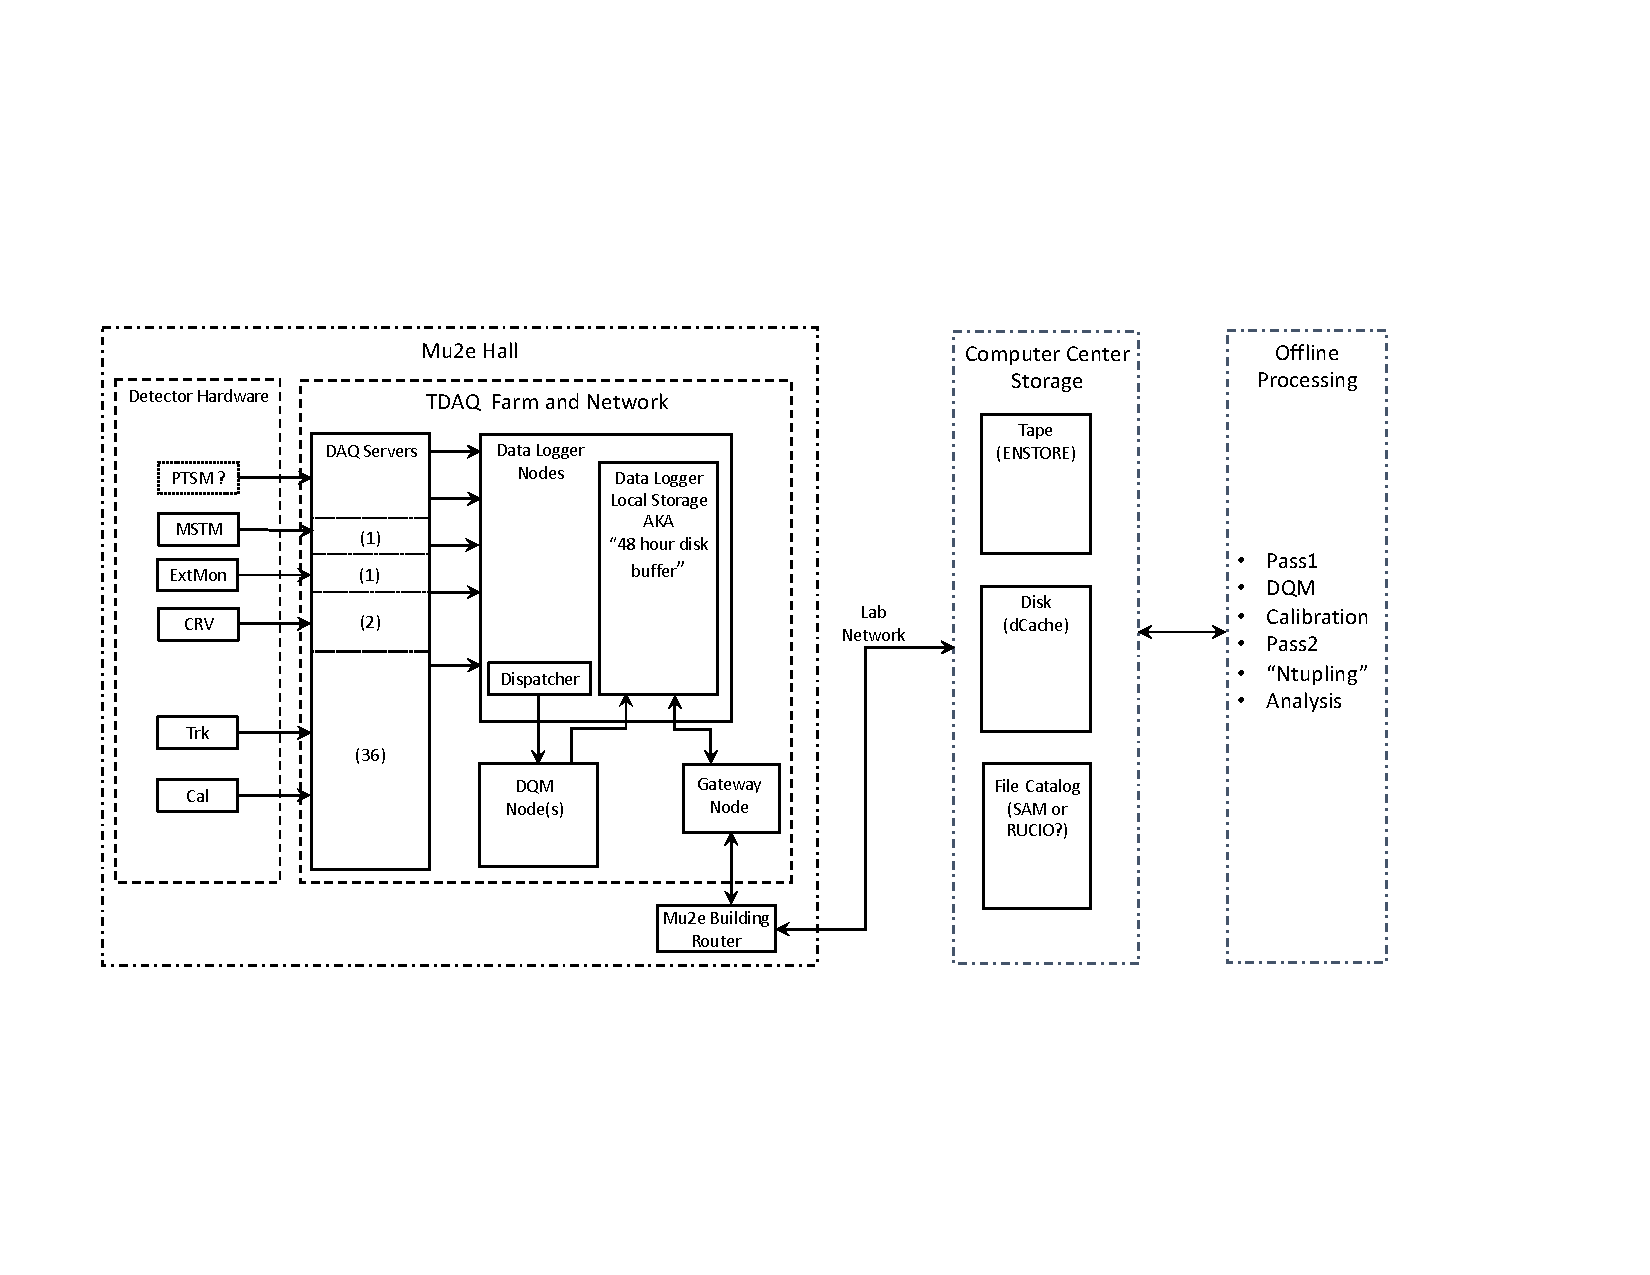
\includegraphics[width=0.9\textwidth]{figures/interface_with_TDAQ.pdf}
\caption[Block diagram of interfaces seen by the Mu2e RDM]{
  Block diagram of the world seen by the Mu2e RDM.
  See the text for a discussion of these elements.}
\label{fig:blockdiagram}
\end{figure}

Data flows from the detectors, through the DAQ system into the TDAQ computer farm.
The five approved detectors are the Tracker (Trk), Calorimeter (Cal), the Cosmic Ray Veto system (CRV),
the Muon Stopping Target Monitor (MSTM) and the downstream Extintion Monitor (ExtMon).
A sixth detector has been proposed, the Production Target Scanning Monitor (PTSM),
which is drawn with a dotted box;
it's primary use is to send rapid feedback to the accelerator control room
and it's not clear what, if any, data it will send through the TDAQ system.
In any event the data volume from that PTSM will be small enough that it will not be
a driver for the RDM.

A cartoon picture of the TDAQ computer farm is that it has 40 DAQ Server nodes
that talk to the detectors, build events and run trigger algorithms on those events.
The design is a deadtimeless streaming DAQ system that has no hardware trigger;
it reads every event from the detector hardware and sends all events to software filters
that run on the DAQ server nodes;
the software makes the trigger decision.
The present design is 20 software filter processes on each of the 40 DAQ server nodes, 800 total.
Events that pass the trigger are forwarded to Data Logger nodes that will write the events
to files in the Data Logger Local Storage (DLLS), a RAID 0 hybrid SSD/HDD array on the bus of the Data Logger nodes.
Appendix~\ref{app:DataLoggerLocalStorage} has the specs for and a discussion about this disk array.
In earlier DPC related talks and documents this was refered to as the ``48 hour disk buffer''.
In addition to the triggered events, a variety of prescaled, untriggered events will pass the
trigger and be handled the same as events that passed the trigger.
Finally, there will be special data streams for calibrations.

The base design is to have a two data logger nodes that receive the data from all DAQ server nodes
and write it to files in the DLLS.
The data logger nodes will write several files, each containing events selected by a different algorithm.
Details can be found in Chapter~\ref{ch:DataStreamsAndFileStreams}.

The Data Logger nodes will also have a process called a ``Dispatcher''
that requests events from the {\code artdaq::DataLogger} processes
and forwards them to clients.
The Dispatcher is designed to exert no back pressure on the {\code artdaq::DataLogger} processes
and, therefore, will normally see only a subset of the events.
Two of the clients foreseen for the Dispatcher are an Event Display and
a Data Quality Monitoring (DQM) system,
which will produce histograms, timelines etc that can be viewed in real time.
Periodically the DQM system will write it's histograms, log files etc to
files in the data logger local storage.  One of the jobs of the RDM will be
to move these files to long term storage.

All of the computing resources in the TDAQ farm are on a private subnet
and cannot been seen from the lab network.  Access in and out
of the private subnet will be via a gateway node that is connected to
both the private subnet and the lab network.
Purchasing and maintaining the gateway node is the responsibility of the TDAQ group.

When the Mu2e Hall was built and provisioned, CCD personnel installed a dual router
and connected it to the lab optical fiber network.
RDM will move data from the Mu2e Hall
to the computer center using this router and the lab optical fibre network.
The router is standard item that CCD uses in many places around the lab; it stocks spares.
CCD is responsible for the maintenance of both the router and the network.
See Appendix~\ref{app:RouterAndNetwork} for additional details of the arrangement with with CCD,
including costs that must be paid by Mu2e to CCD for this service.


For the foreseeable future Mu2e expects that the disk and tape services provided
by SCD will be dCache and ENSTORE.
At this writing Mu2e is using SAM as the file catalog system for files produced
by simulations, tests stands and Vertical Slice Tests (VST).
SCD plans to phase out SAM and replace it with a more modern system, RUCIO \fixme{reference};
RUCIO is already in use by CMS and by DUNE for proto-DUNE Single Phase data.
It is likely that SAM will be phased out during the lifetime of Mu2e.
One of the questions to ask in the design of the RDM is
when to make the transition to RUCIO.

\fixme{Say something about Pass1 and follow-on elements of the offline processing.}

\section{The EventWindowTag and the EventMode}
\label{sec:EWTagAndEventMode}

The heart of the TDAQ system is the Clock Fan-Out (CFO) that delivers
configuration information and timing signals to all elements of the DAQ.
Just prior to the start of each event, the CFO distributes a configuration packet
that describes the upcoming event;
this includes two elements that will be discused below.

\fixme{Ask Ryan what the right name for configuration packet is.}

An event window is defined as time interval during which the DAQ collects data for one event.
Each event window is identified by a 48 bit field in the configuration packet, called
the Event Window Tag (EWT);
the EWT will be monotonically increasing throughout the Mu2e experiment and
enough bits have been reserved for it to produce unique identifiers for all
events over a many-year run.
The CFO is responsible for incrementing the EWT and putting the correct value into
the configuration packet for each event.
The detector readout electronics label information from their subsystem with the EWT,
which is later used as the key for event building.

The Mu2e detector can operate in several modes, two of which,
on-spill and off-spill, will be discussed in the next section.
In addtion there will be several calibration modes.
All elements of the TDAQ have pre-programmed operations defined for each mode.
When the CFO creates the configuration packet for each event,
it sets a bit field called the EventMode (EM)
that tells the TDAQ system in which mode to operate for the upcoming event.

\section{On-Spill, Off-Spill and Near-Spill}

This section defines the concepts of on-spill, off-spill and near-spill running.

It is expected that, for most of it's running time,
Mu2e will share parts of the Fermilab accelerator complex with a neutrino experiment,
first, with NOvA and, later, with DUNE.
To keep this document easier to read it will discuss sharing with NOvA but sharing with DUNE is implied.
The change from NOvA to DUNE may change details
but will not materially change the requirements of the RDM.

Sharing with NOvA drives the repeating cycle of Mu2e operations, a Main Injector (MI) cycle of
21 Booster (BO) cycles.
The duration of one Booster cycle is 1/15~s,
making the duration of one MI cycle 1.4~s.
Figure~\ref{fig:beamMacroStructure} shows a cartoon of the MI cycle.
From the Mu2e point of view, the cycle starts with a series of 8 slow spills
from the Delivery Ring (DR) to the Mu2e production target;
within each spill, proton pulses arrive at Mu2e every 1695~ns;
the duration of a spill is nominally 25,438 pulses, about 43.1~ms.
There is a gap of about 5~ms between spills.
The eigth spill is followed by a period of about 1020~ms,
during which no proton pulses arrive at Mu2e;
during this time, beam is delivered to NOvA
and beam is prepared for the next 8 spills to Mu2e.
Then the cycle repeats.

\begin{figure}[tbp]
\centering
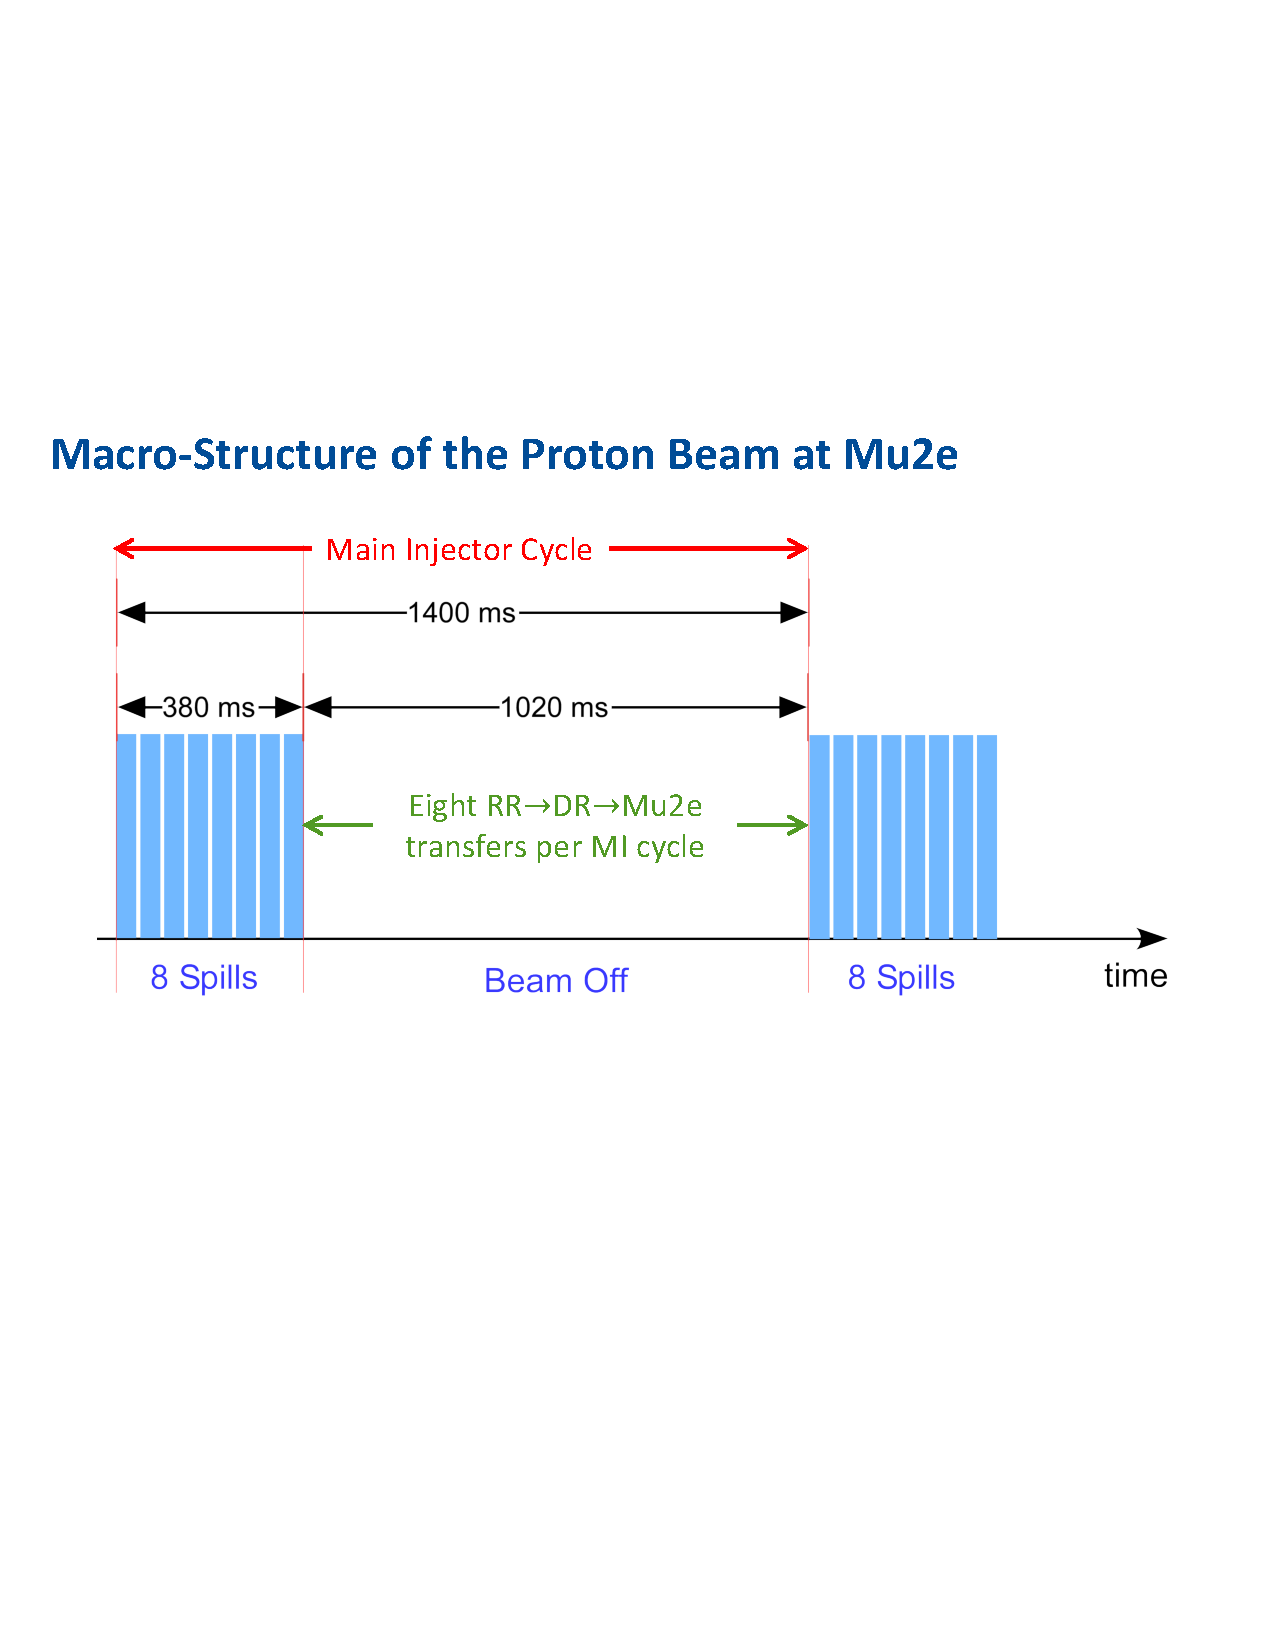
\includegraphics[width=0.9\textwidth]{figures/ProtonBeamLongitudinalStructure2019-01-10_page6.pdf}
\caption[MacroStructure of the Proton Beam at Mu2e]{
  MacroStructure of the proton beam at Mu2e, taken from page~6 of
  the file ``Proton Beam Longitudinal Structure (.pdf)'' from
  Reference~\protect{\cite{beamTiming}}.  The figure is described in the text.}
\label{fig:beamMacroStructure}
\end{figure}

During the spills, Mu2e is running in the on-spill configuration.
During the 1020~ms no-beam period, Mu2e is running in the off-spill configuration.
These two configurations are discussed below.
It has not yet been decided if the 5~ms periods between spills will
be in the on-spill or off-spill configuration
but that does not materially affect the design of the RDM.
Table~\ref{tab:timescales} summarizes the time scales within one MI cycle.
\begin{table}
\begin{center}
\caption[Properties of the Beam-to-Mu2e MI Cycle]{Properties of Beam-to-Mu2e MI Cycle.}
\label{tab:timescales}
\begin{tabular}{ll}\hline
   1/15~s & Period of one Booster cycle \\
   21     & Booster cycles within the MI cycle \\
   1.4~s  & Period of one MI cycle \\
   43.1~ms & Duration of one spill \\
   8       & Number of spills per MI cycle \\
    5~ms   & Duration of the period between two spills \\
   1020~ms & Duration of the off-spill period within one MI cycle \\
   1695~ns & Period of the Delivery Ring and the duration of one on-spill event\\
   100~$\mu$s & Duration of one off-spill event \\
   24.6\%     & Duty factor (total spill time divided by MI cycle duration)\\
   \hline
  \end{tabular}
\end{center}
\end{table}


In the on-spill configuration, one event will have  a duration of 1695~ns
and it records the information associated with one proton pulse.
The trigger will be configured to select interesting events associated with the proton pulse
and to pre-scale non-triggering events in order to study the performance of the trigger.
In the off-spill configuration, one event will have a duration of 100~$\mu$s.
During the off-spill period, Mu2e will trigger on cosmic rays that
pass through the tracker and/or the calorimeter; it will also collect
pedestal data from some of the subsystems; some calibration procedures
may also take place during the off-spill period.

Mu2e expects that the accelerator super-cycle will consist of a
sequence of many of the above MI cycles,
with an occaisional other cycle mixed in.
For example, when MTEST is active, there is usually beam delivered to MTEST about once per minute.
When this occurs, Mu2e will have an extended period of off-spill running.

There will also be periods in which the accelerator complex is not delivering
beam to Mu2e for an extended time, minutes, hours, days or weeks.
In some of these periods Mu2e will shutdown to perform maintenance, repairs or upgrades;
in others Mu2e will execute calibration runs;
and in others Mu2e will collect data in off-spill mode for an extended period of time.


The Mu2e TDAQ team have defined a value of the Event Mode that they have named near-spill.
This is to allow for the possibility that some subsystems may want to
configure themselves differently during the transition from on-spill to off-spill.
At this time there are no definite plans to use this mode but it is available if needed.

The design of the Mu2e TDAQ system is that trigger processing lags the incoming events
during the on-spill period and catches up during the off-spill period.  There is
buffering at various places in the TDAQ system to support this.

It's possible that the MI cycle might need to be increased to 22 BO cycles;
should that happen the additional time will be allocated to a longer off-spill period.
Also, Mu2e plans to start operations with a slightly different configuration:
4 spills instead of 8, with each spill of a longer duration than 43.1~ms;
this mode is called ``one bunch'' running or ``Phase~1'' running.
Neither of these materially changes the requirements for the RDM and
will not be discussed further.

There will be times when Mu2e is taking data but NOvA is not.
In such times, the base plan is that Mu2e will continue to take data using the same MI cycle of 21 BO cycles.
There are several technical reasons that prevent Mu2e from reducing the off-spill period
in order to increase the duty factor.\footnote{
There are radiation safety limits on the average beam power;
the production target will have a reduced lifetime at higher average beam power;
the TDAQ system cannot accomodate a signficiantly higher event rate because it
uses the off-spill period to catch up on buffered events.
\fixme{These might not apply during one bunch running; so we could see a shorter MI cycle
during one bunch running.}
}

\section{EventIDs, Runs and Subruns}
\label{sec:TagsIDsRunsSubRuns}


Mu2e uses the \art event processing framework;
the trigger filter processes that run in the trigger farm will each be a separate \art process;
\art will also be used for offline data processing.
In \art, events are uniquely identified by a 3 part identifier called an
{\code art::EventID}; the parts are named run number, subrun number
and event number.

Within the DAQ system, event fragments and fully assembled events
are identified by the Event Window Tag (EWT).
The DAQ system will translate each EWT to an {\code art::EventID}
before events are presented to the \art based software filter processes.
The mapping of EWT to  {\code art::EventID} will be unique and
{\code art::EventID}'s will be monotonically increasing with the time
that the event ocurred.
The EWT will be recorded as part of the \art data for each event.


\fixme{ So far as I know the mechanics of mapping EWT to EventID
  is only captured in an email thread.
  Is there a real reference?
  If not, who will write it up in a referenceable way?
}

The meaning of run and subrun are defined by Mu2e.
All that \art requires is that a subrun contain zero or more
events and that a run contain zero or more subruns.

The current plan is that runs will typically have a duration of a few hours
while subruns will contain an integer number of MI cycles and
have a duration somewhere between 14 seconds and a few minutes.
This means that each subrun will contain both on-spill and
off-spill events.
The transition between subruns will happen during the off-spill period,
in order to ensure that each on-spill period is contained within a single subrun.

These durations are informed by the following.
Mu2e has designed a conditions management system
in which intervals of validity (IOV) are a specified as a range of subruns;
such a range may either span runs or be contained within a single run.
Therefore subruns must be short enough to follow the most
rapidly changing conditions.  As of this writing it seems
likely that the upper limit for the duration of a subrun will
be driven by data handling and downstream data processing;
that is, files should be neither too big nor too small
and the follow-on data processing jobs should be able to process one subrun
in, at most, a few hours.

The Mu2e TDAQ has been designed so that subrun transitions will be deadtimeless
but that data taking will pause for a few minutes at run transitions.
At each run transition the TDAQ system will do some house keeping,
including resetting some hardware, reloading some firmware and restarting some processes.
These steps are designed to cure any Single Event Upsets (SEU) in the firmware
and to generally ensure a robust TDAQ system.
Therefore a run should be long enough that the deadtime
caused by the run transition is a small fraction of the total run time
but short enough that the resets occur frequently enough
to keep the system robust.

Anomalies that occur during data taking will cause some runs
and subruns to be cut short.  Therefore the RDM must sometimes
expect smaller files, perhaps even empty files.


\section{Organization of Data by Detector Subsystem }
\label{ssec:dataOrganization}

This section will give an outline of how data from the
various detector subsystems flows from the detector to the DLLS.
This will help explain why the data organization in the DLLS is what it is.
The text in this section refers to Figure~\ref{fig:filesDLLS}.
These descriptions are only high level overviews,
intended to convey enough information to design the RMD and no more.

\fixme{References to the full story.}

\begin{figure}[tbp]
\centering
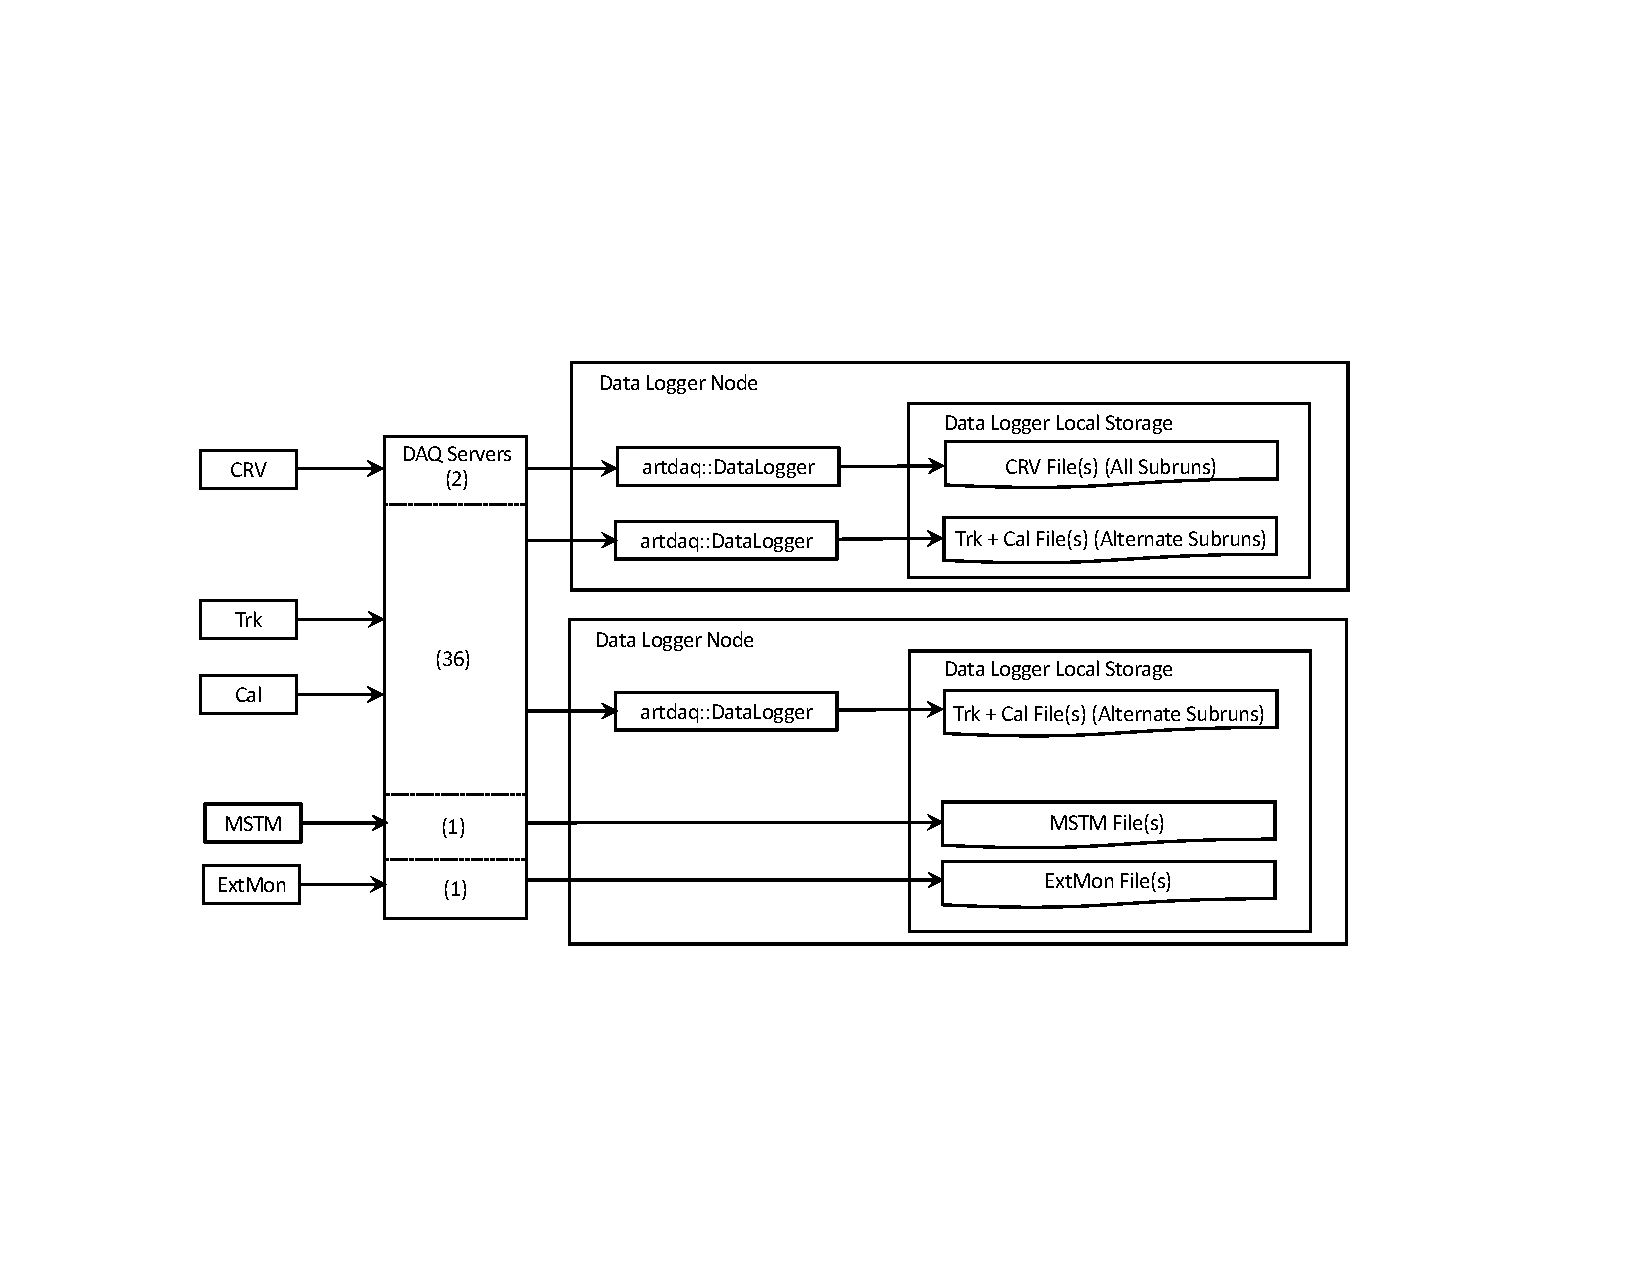
\includegraphics[width=0.9\textwidth]{figures/FilesInDLLS.pdf}
\caption[Files in the DLLS]{
  Files in the Data Logger Local Store; the figure is described in the text.}
\label{fig:filesDLLS}
\end{figure}


\subsection{Tracker and Calorimeter}
\label{ssec:TrkAndCal}

Data flows from the tracker and calorimeter into FPGAs mounted the PCI-e bus of 36 of 40 DAQ servers;
these FPGAs are called Data Transfer Controllers (DTCs).
All DTCs on these 36 DAQ servers communicate with each other over a high speed switch
and perform event building.
Event building uses only resources from the DTCs and is indepdent of operations on the host DAQ servers.
The end product of event building is that each DTC contains buffers of complete events held in its own memory;
each event is complete in the sense that it contains all of the data from the tracker and calorimeter
but it does not contain any data from other subsystems.
Every event is present in exactly one buffer and each DTC sees only a small subset of the full event stream.

Once a DTC has a full buffer of events it will transfer that buffer to its host DAQ server;
it does so by transfering it to an {\code artdaq::BoardReader} process.  On most of the
36 DAQ severs there are two DTCs and two {\code artdaq::BoardReader} processes;
on the remaining servers there is one DTC and one {\code artdaq::BoardReader} process.

The 20 trigger filter \art processes on each DAQ Server are controlled by a process
called an {\code artdaq::EventBuilder}.
This name is historical and reflects the function that it had for the previous experiments in which \artdaq was developed.
For Mu2e, event building was done in the DTCs and the function of an
{\code artdaq::EventBuilder} process is to receive events from one of
the {\code artdaq::BoardReader} processes and to distribute them to the trigger filter \art processes.

If an {\code artdaq::EventBuilder} has trigger filter processes that are ready for their next event,
and if no events are available from {\code artdaq::BoardReader} process(es) on that server,
then the {\code artdaq::EventBuilder} can fetch event buffers from {\code artdaq::BoardReader} processes
on other DAQ servers.
This allows all 40 DAQ servers to run trigger filter processes even though only 36 of the 40 servers
communicate with the tracker and calorimeter.

The end result is that each event will be seen by exactly one of the 800 trigger filter processes.
Within one trigger filter process there is no guarantee that events within one subrun will arrive in
increasing order of {\code art::EventID}.

\fixme{Is there a guarantee that, within a single process all events from subrun n will be seen before
any events from subrun n+1?  If so, for personal interest, how is this guarantteed?}

The trigger filters process the events and make a trigger decision on
each event.
The current design is that about 1 in 400 events will pass the trigger;
this includes all events that pass the primary triggers,
pre-scaled events that pass the secondary triggers,
pre-scaled events that fail at selected places during trigger processing,
and random triggers.
Throughout this document the phrase ``passes the trigger'', without additional modifiers,
refers to all of the above, including the prescaled events and random triggers.
The trigger rate is dominated by pre-scaled secondary triggers,
which are primarily used for calibration and monitoring.

\fixme{Define primary and secondary triggers. Or reference where it is defined.
  Is this language used elsewhere? If so, use the language.}

Each \art trigger filter process sends events that pass the trigger over a standard ethernet
to one of the two data logger nodes where they are received by an {\code artdaq::DataLogger} process
that writes the events to files in the DLLS.
This process may be configured to write all events to a single file
or to split the events across several files,
for example all on-spill to one file and all off-spill events to another.
The details are to be determined.

Because different events have very different processing times in the trigger processes,
and because {\code artdaq::EventBuilder} processes can draw events from
any of the {\code artdaq::BoardReader} processes, events will arrive at the
{\code artdaq::DataLogger} out of order.  In particular, early events from subrun N+1
may arrive at the {\code artdaq::DataLogger} before the last event from subrun N.

The TDAQ base design has two Data Logger nodes, each running an
{\code artdaq::DataLogger} process that will receive tracker and calorimeter events.
The plan is to send events from alternate subruns to each of the two.
This allows a clean separation of the event stream into non-overlapping subruns.
Within a each subrun, however, the events may not be in order.

\fixme{If we end up with short subruns, say 10 MI cycles, 14 s, will we need to stripe
  this 3 or 4 wide to survive the longest processing latencies?}

The above story is almost exactly the same for both on-spill and off-spill running.
One difference is that the trigger filter processes test the EventMode
and run different algorithms for the two cases;
the other difference is that the rate of triggered events
and data volume per triggered event will be much smaller in off-spill than in on-spill events.


The behaviour for other event modes will be discussed elsewhere.
\fixme{Add references}

\subsection{Cosmic Ray Veto}
\label{ssec:CRV}

In on-spill running,
data from the CRV system is read from the detectors and held in buffers in the
readout electronics chain.
When one of the trigger filter processes described in the previous section
decides that an event has triggered,
it sends a message to the CRV system and requests that information from that
event be forwarded to a Data Logger node.
The requested information flows from the readout electronics through 2 two of the 40 DAQ servers
to a third {\code artdaq::DataLogger} process that is running on one of the Data Logger nodes.
This third {\code artdaq::DataLogger} process writes the events to files in the DLLS.
Again, this process may be configured to write all events to a single file
or to split the events across several files,
perhaps on-spill to one file and off-spill to another.
The details are to be determined.

\fixme{where are the buffers? ROC? FEB?}

The end result is that each event in the DLLS will be split across two files, one with the
tracker and calorimeter data and one with the CRV data.
One of the questions to be answered when designing the RMD will be to identify
the point in the workflow that these two event fragments will be joined into one.
That point could be within the RMD or within Pass1.

The original design of the TDAQ was the that an {\code artdaq::DataLogger} process
would receive the tracker and calorimeter information
and buffer that internally until the CRV information arrived.
After that information arrived,
the {\code artdaq::DataLogger} process would write an event containing information from all 3 subsystems.
Recently the TDAQ team became concerned that this scheme would not work because
the tail to long processing times in the trigger filters would exceed the buffering capacity within
the CRV readout electronics.
Therefore this plan was replaced with the one described earlier.


The light sensors for the CRV system are Silicon Photomultipliers (SiPMs).
The CRV team have requested that, during off-spill running,
TDAQ acquire as large a sample of SiPM noise as is practical;
they will use this data to study the time dependence of the SiPM pedestals.
This data is sometimes called ``SiPM noise'' or ``SiPM pedestal data''.

Mu2e will automatically get a small sample of SiPM noise from the off-spill events
that trigger based on tracker and calorimeter data.
However this trigger rate will be only a few Hz, which will not yield enough SiPM noise.
One option is for the trigger filters to pre-scale failing off-spill events at a rate that will
produce a large enough sample of SiPM noise.
In this case the events in the SiPM noise events will include information from the tracker and calorimeter
(albeit in separate files).
A second option is for an indepedent agent within the TDAQ system to trigger the SiPM noise events;
in this case most SiPM noise events will usually not contain tracker and calorimeter information.
The TDAQ team has not yet decided between these options.

\fixme{The collaboration should ask for the first option if that's what they want.}

\subsection{Extinction Monitor}
\label{ssec:ExtMon}

The Extinction Monitor system sends its data to a single node in the DAQ server farm.
That server will receive the data and write it directly to one or more files in
the DLLS.  This server will also have trigger filter processes that receive
data from buffers on the 36 servers that talk to the tracker and calorimeter.

\fixme{confirm that there are no {\code artdaq::DataLogger} proccesses involved and
that the DLLS is nfs mounted to this server.}

\subsection{Muon Stopping Target Monitor}
\label{ssec:ExtMon}

The Muon Stopping Target Monitor sends its data to a single node in the DAQ server farm.
That server will receive the data and write it directly to one or more files in
the DLLS.  This server will also have trigger filter processes that receive
data from buffers on the 36 servers that talk to the tracker and calorimeter.

\subsection{Production Target Scanning Monitor}

The principle client for data from the PTSM is the accelerator control room.
At this writing it has not yet been defined if it the PTSM will write any data the the DLLS.
Should that happen it is likely that the pattern will be the same as for the ExtMon
and MSTM.


\chapter{Data Streams and File Streams}
\label{ch:DataStreamsAndFileStreams}

This chapter defines the ideas of ``data streams'' and ``file streams''.
It enumerates the data streams that are anticipated at this time
and it presents a strawman for how these may be grouped into files.

\fixme{Should I use the word ``dataset'' instead of ``file stream''?
  I am using a distinct word for now since I want to reserve the word
  of dataset for something that is defined using SAM.  Are these
  two ideas identical?
}

A ``data stream'' is a series of events selected by some algorithm;
one attribute of events in a data stream is they all require the same downstream processing.
For example the on-spill and off-spill events are distinct data streams.
The on-spill events will have many trigger lines; one might consider each trigger
line it's own data stream or one might define groups of trigger lines as a data stream.
Another example: the off-spill events will include some events that triggered based on
the tracker or calorimter and they will also include events that did not trigger but
which are retained to collect a sample to study pedestals in the CRV system.
These are distinct data streams.

A ``file stream'' is a series of files that contain events from one or more data streams.
For example we might decide to bundle all of the on-spill data streams into a single
file stream or we might decide to put some of the on-spill data streams into one file
stream and another set of on-spill data streams into a different file stream.
For example all of the files containing off-spill events might be one file stream;
or maybe we will decide to split the off-spill events in to
the two off-spill data streams into two file streams.

The key point is that data streams are a fundamental idea,
while file streams are choice about how to group data streams for convenience of data handling and downstream processing.

\fixme{We need to address if a given event may be in more than one data stream.
       And we need to address if a given data stream may be in more than one file stream.
}

% Example
% Keep sections under development
\IfStrEq{\ISDRAFT}{YES}{

\chapter{A Chapter under development}
\label{ch:under_development}

This is a chapter still under development.
It is kept here to illustrate the use of the  ISDRAFT macro.

} % end `ISDRAFT = YES'

\chapter{Requirements}

This chapter lists requirements for the RDM system.
The requirements are dervived from the above firehose of information.

\begin{enumerate}
  \item Move data in a timely fashion; goal is that Pass1 will be complete within 6 hours of file close 95\% of the time.
    \fixme{check 6 hours}
  \begin{enumerate}
    \item When a backlog occurs, for example, during scheduled dCache maintenance, prioritize which files go first.
    \item The DAQ may produce some files that need to travel in pairs, for example Trk+Cal on-spill and CRV on-spill.
  \end{enumerate}
\item Manage free space in the data logger local storage to ensure enough space for at least \fixme{ ??} more
  hours of data taking.
\item Provide a way to monitor the status of the RDM;
  the monitoring system should automatically raise warnings an alarms when appropriate.
\end{enumerate}

\chapter{Questions}

A list of questions that should be addressed in the design of the RDM:

\begin{enumerate}
\item Start by sticking with SAM and move to RUCIO later?  Or move to RUCIO now?
  How does this decision interact with requirements for ongoing simulation, VST
  and test stand work?
\item Work with TDAQ to understand the constraints that drive the choices of how to
  map data streams to file streams.
  \begin{enumerate}
    \item a separate filestream for the intensity stream.
    \item split on-spill and off-spill to separate file streams
    \item split off-spill into triggered and pedestal.
  \end{enumerate}
\item Identify where in the workflow the split raw data files, Trk+Cal in one,
  and CRV in the other, will be joined into a single file.  This will require consultation with the team running
  Pass1.
\item In the event of multiple data loggers, when do the files from a single subrun get joined to atomic.
\item Check with TDAQ: will you close an output file every subrun and open a new one? Will it be the same
  on all file streams or can it differ?  What's the plan to deal with a subrun transition when one
  event is very late arriving?  How does that last case affect RDM?
\end{enumerate}


\appendix

\chapter{Network Between Mu2e Building Router and Computer Center}
\label{app:RouterAndNetwork}.

The Mu2e building router is owned by CCD.
\begin{itemize}
\item specs; dual; auto fail over; channels; free to increase \#channels
\item Router is owned and maintained by CCD; stock item so they can replace quickly.
\item We pay yearly maintenance: \fixme{Amount in FY21 and inflation estimate}
\item We pay for replacement; we pay CCD and they do the work. \fixme{when is next replacement due; replacement cycle}
\item \fixme{make sure this is in MOU} Coverage.
\item \fixme{not sure who paid for the existing one.}
\end{itemize}


The lab network.
\begin{itemize}
\item Install and maintained by CCD.
\item Normal maintenance and repair is budgeted for in their ops budget
\item If there were an emergency repair that exceeded their budget they would come to us. \fixme{make sure this is covered in MOU}
\end{itemize}

\chapter{Data Logger Local Storage}
\label{app:DataLoggerLocalStorage}

\fixme{ Specs etc on the Data Logger Local Storage go here}.

\chapter{Things to Know About \art}

This chapter describes details of \art that should be considered when
designing the RDM.  This includes details that are important for the RDM
proper and details that are important when shaping data for downstream
processing.

\section{Atomic Subruns}
\label{sec:AtomicSubruns}

A subrun is said to be ``atomic'' if all of the events in that subrun are found in a single \art file.
If subruns are atomic, some bookkeeping operations are simplified and Mu2e plans to exploit this;
therefore the TDAQ and RDM should aim to create atomic subruns as early as possible in the workflow.

Why ``as early as possible'' and not ``must''?

The base design of the TDAQ is to have one {\code artdaq::DataLogger} process that will
see all events and write them to disk; it may write several output files.
However it is possible that a single {\code artdaq::DataLogger} will not have the
resources to handle the load.  Should that happen the solution is to have two
{\code artdaq::DataLogger} processes, each of which sees about half of the events.
In this case all of the output files will be duplicated,
one for each {\code artdaq::DataLogger}.
In this case subruns are not atomic;
the RDM and DPC will need to work together to decide where in the workflow these two files
are joined to create atomic subruns.

There is an additional subtlety.
Section~\ref{sec:TagsIDsRunsSubRuns} described that Mu2e subruns will cover many MI cycles
and, therefore, will include both on-spill and off-spill events.
One option for the TDAQ, the option that is preferred by DPC,
is that TDAQ will write on-spill and off-spill events to separate files.
The Mu2e DPC anticipates only workflows in which these two files are treated separately;
another way of saying it is that there will be no jobs that read events from both of these files.
Therefore we can say that within each of these two file streams the design is for subruns to be atomic.
This is the usual meaning of ``atomic subrun'' throughout this document.

\subsection{Sparse Skims}

This section assumes that the reader is familiar with the \art concepts
of data products that are held by the {\code art::Run} object
and data products that are held by the {\code art::SubRun} object.
It also assumes that the reader is familiar with the \art concepts
of {\code art::Run} and {\code art::SubRun} fragments
and with the concept of aggregation for these fragments.
For information about these concepts see~\cite{RunAndSubRunProducts}
and~\cite{ProductAggregation}.


By default \art assumes that subruns are not atomic
but you can tell \art that subruns will be atomic by adding this fcl
parameter to the parameter set of the RootInput module

\cmd{ compactEventRanges : true}

When \art sees a beginRun transition, it reads all run data products from the input file.
When \art is configured for atomic subruns, it drops these data products
from memory at the matching endRun transition.
Similarly, when \art has beginSubRun transition, it reads all subrun data products from the input file.
When \art is configured for atomic subruns, it drops these data products
from memory at the matching endSubRun transition.
When \art is not configured for atomic subruns it does not drop these data products from
memory at the matching endSubRun transition; the reason is that 

On the otherhand, when art is configured for non-atomic subruns

When \art is configured for non atomic subruns there is an extra memory cost;
for sparse skims this can dominate the memory usage of the process.
While this added memory cost is small early in the production, chain when
only a few subruns are seen by any given process, it's important to be
aware of this constraint when shaping the data for downstream processing.

To understand how the memory cost arises,
it is necessary to understand the structure of an art file.
Suppose that you have an art file with run:subrun ( 1:1, 1:2, 2:1, 2:2).
When you read the art file you will see the sequence of records shown
in table~\ref{tab:atomicsubruns}.

\begin{table}
\begin{center}
\caption[Example For Discussion of Atomic Subruns]{Example for the Discussion of Atomic Subruns}
\label{tab:atomicsubruns}
\begin{tabular}{l}\hline
  begin run record for run 1 \\
  begin subrun record for subrun 1:1 \\
  records for the events of subrun 1:1 \\
  end subrun record for subrun 1:1 \\
   begin subrun record for subrun 1:2 \\
   records for the events of subrun 1:2 \\
   end subrun record for subrun 1:2 \\
   end run record for run 1. \\ \hline
   begin run record for run 2. \\
   begin subrun record for subrun 2:1 \\
   records for the events of subrun 2:1 \\
   end subrun record for subrun 2:1 \\
   begin subrun record for subrun 2:2 \\
   records for the events of subrun 2:2 \\
   end subrun record for subrun 2:2 \\
   end run record for run 2. \\
   \hline
  \end{tabular}
\end{center}
\end{table}

Now suppose that your job reads the run and subrun scope data products at begin run/subrun time.
If \art is configured for atomic subruns, after processing the module and service
{\code endSubRun} calls, it will delete the subrun data products from memory. It can safely do this
because it knows that it will never see another event from that subrun.
Similar for the run scope data products.

On the other hand, if \art has been configured for non-atomic subruns, it will retain all subrun
and run data products in memory until the end of the job.
For a job that sees a small number of subruns this is usually not an important memory cost; but
for sparse skims it can be dominant.


There is a second consideration about atomic subruns:
for sparse skims there is signficant memory savings if subruns are atomic.
While the RDM will not see sparse skims, the people developing it should know the big picture.


\section{Order of Events}

\chapter{Risk Registry}
\label{app:RisKRegistry}

\section{Split Files from DAQ}
\label{app:Risk:SplitFiles}

The base design is to have a single data logger node that receives data from all DAQ server nodes.
This design cannot be tested at scale until all of the hardware has been purchased;
even then, the tests will be based on simulated events, not actual data.
There is a risk that there will be a bandwidth limit that makes this impossible.
Should this occur, there backup plan is to have two or more Data Logger nodes
that each see a fraction of the events;
perhaps half of the DAQ Servers talk to one Data Logger node and the other half talk to another node.
The result will be that events from the same file stream from the same subrun end up split across multiple files.
This breaks the requirement that subruns be atomic.

Should this occur the RDM will need to modify the bookkeeping system to allow non-atomic subruns early
in the workflow and modify the workflow to restore atomic subruns as soon as possible.

Another alternative is to tighten the trigger algorithms to accept fewer events;
this risks loosing events that we really do want to keep and is the last alternative.

\clearpage
\phantomsection
\addcontentsline{toc}{chapter}{Bibliography}
\printbibliography


%\cleardoublepage
%\printindex
